% REV_P0 2026-11-24：由 chapter_04_results_rewrite_v1_20261122.tex 派生；V1保持不变。
% 新增数值全部来自 REV_P0_20261124/derived/T1–T8（既有CSV只读汇总；posthoc列已标注）。
% 本轮不新增实验，不改变任何预测或冻结结果；所有负结果保留并补充。
% 第三篇CellCharter毕业论文第四章结果与分析：2026-11-22首版重写
% 本稿为论文写作草稿，待导师确认章节编号、全论文术语、图件排版。
% 证据入口：RESULTS_ARCHIVE_STATUS_20261122.md
% 不改写任何实验数据；2026-11-22后的E3d后验ARI/NMI及E3b容差均为明确标记的post-hoc分析。
% 警告：如在主文件中用\chapter{...}引入本稿，请调整本文件首行section层级。
\section{实验结果与分析}
\label{sec:cellcharter-results-v1}

\subsection{评价任务、数据结构与报告口径}
\label{subsec:cellcharter-design-v1}

本章围绕空间转录组聚类结果的三个问题开展实证分析：多尺度邻域表征的深度是否影响空间域划分，无标签聚类数选择是否改变性能评价，以及聚类质量与空间边界定位之间是否存在不同的变化趋势。在此基础上，本章加入成熟聚类方法对照和独立组织队列评价，以检验相关观察在不同样本中的适用范围。研究使用CellCharter已实现的多尺度邻域特征聚合与聚类流程，对已有表征进行固定组合、累计深度和聚类数设置比较；不将特征重组表述为新提出的基础聚类算法。

主要DLPFC数据包含12张Visium切片，分别来自3位供体，每位供体4张切片。以切片为单位计算聚类评价，以供体作为独立生物学来源；同一供体的4张切片与同一切片的不同技术种子不能视为独立生物学重复。外部评价采用6例乳腺癌患者对应的Visium数据；其中6名患者是独立生物学样本。各分析的均值均明确注明其汇总层级，不对切片、spot、空间边或随机种子实施伪独立统计推断。

聚类结构评价使用调整兰德指数（adjusted Rand index，ARI）和归一化互信息（normalized mutual information，NMI）。其中NMI为算术平均归一化形式。仅在人工参考标注可用的spot上计算两项指标。空间边界评价使用Visium阵列坐标所定义的六邻接无向边，仅保留两个端点均有有效参考标签的边；参考边界定义为相邻spot属于不同参考层，预测边界定义为相邻spot被分入不同原始聚类编号。严格边界F1由真正例TP、假正例FP与假负例FN计算：
\begin{equation}
F_{1,\mathrm{strict}}=\frac{2TP}{2TP+FP+FN}.
\label{eq:cellcharter-boundary-v1}
\end{equation}
严格指标要求预测边界与参考边界在同一图边上完全一致。后验敏感性分析另行考察1-hop、2-hop容差：在有效无向边构成的线图中，以边到边距离定义容差，并以一对一最大基数匹配防止重复将多个预测边界计为同一真实边界的TP。容差F1反映邻近检出，而非严格的边界定位精度，三种结果必须分别报告。

本章区分两种聚类数策略。Oracle-K使用人工参考层的类别数决定K，属于标签类别数知情的评价条件，不等同于无标签模型选择；K-blind不使用参考标签决定聚类数，其标签仅用于预测文件冻结后的后验评分。本研究不将Oracle-K自动视为所有指标的理论上界，也不将不同K选择方式产生的结果混为一组。DLPFC早期开发切片、补充分析及新增的外部队列之间的关系依各阶段原冻结协议解释；本章所有新增后验分析均保留其发生于原模型训练完成之后的时间顺序。

\subsection{多尺度邻域特征与固定K条件下的聚类表现}
\label{subsec:cellcharter-e1e2-v1}
% 数据来源：E1E2_20261119_RELEASE/derived/all_120_condition_stats.csv
% 以及E1E2_20261119_RELEASE/derived/B_vs_A_12slices.csv

首先，在DLPFC的12张切片上，使用10种事先固定的多尺度特征配置和10个技术随机种子完成1200项GMM聚类评价。累计特征配置从$L_0$（5维）逐步增加至$L_0$--$L_4$（25维），另包括若干固定15维的非连续邻域块组合。本阶段的聚类数依据参考标注类别数设定，因此属于Oracle-K条件，评价的是固定K下的特征组织方式差异，而不是自动选K能力。

将每张切片的10个种子先求平均，再对12张切片作等权描述性平均，累计5D、10D、15D、20D、25D配置的ARI依次为0.3051、0.4081、0.4299、0.4383和0.4418；对应NMI为0.4133、0.5422、0.5780、0.5891和0.5982（表\ref{tab:cellcharter-e1e2-depth-v1}）。

5D到10D的提升幅度最大，而且在12/12张切片和3位供体中方向一致。15D之后，宏平均只略有上升，切片和供体之间方向并不一致：12张切片中有6张的25D ARI低于15D，6张的20D低于15D，5张的25D低于20D；供体D3的ARI依次为15D 0.4648、20D 0.4587、25D 0.4480，方向与宏平均相反。15D之后各深度之间的宏平均差值（0.004--0.012）小于切片间标准差（约0.06--0.07），也与切片内GMM种子标准差（0.023--0.037）处于同一量级。由于增加邻域层同时提高了输入维度，这些变化不能单独归因于邻域传播范围，也不能证明更深聚合在所有样本上都优越。

\begin{table}[htbp]
\centering
\caption{DLPFC固定Oracle-K下累计邻域特征的聚类表现。每切片先平均10个GMM种子，再对12切片等权平均；SD为切片间标准差，种子SD为切片内GMM种子标准差的平均值；D1--D3为各供体4张切片的ARI均值。均为描述性统计，来源REV\_P0表T1}
\label{tab:cellcharter-e1e2-depth-v1}
\small
\begin{tabular}{lcccccccc}
\toprule
累计邻域特征 & 维度 & ARI & SD & 种子SD & NMI & D1 & D2 & D3\\
\midrule
$L_0$ & 5 & 0.3051 & 0.063 & 0.023 & 0.4133 & 0.338 & 0.238 & 0.339\\
$L_0+L_1$ & 10 & 0.4081 & 0.066 & 0.037 & 0.5422 & 0.409 & 0.368 & 0.448\\
$L_0+L_1+L_2$（A） & 15 & 0.4299 & 0.072 & 0.032 & 0.5780 & 0.429 & 0.396 & 0.465\\
$L_0+\cdots+L_3$ & 20 & 0.4383 & 0.060 & 0.027 & 0.5891 & 0.455 & 0.401 & 0.459\\
$L_0+\cdots+L_4$ & 25 & 0.4418 & 0.066 & 0.028 & 0.5982 & 0.475 & 0.402 & 0.448\\
\bottomrule
\end{tabular}
\end{table}

\subsubsection{与CellCharter原作者单切片基准的对照}
\label{subsubsec:cc-official-compare-rev-p0}
25D配置与原作者单切片基准的最终配置相同（表\ref{tab:cc-official-protocol-rev-p0}）。将本研究E1/E2结果与官方仓库发布的逐切片ARI\cite{cellcharteranalyses2024}对照，得到表\ref{tab:cc-official-compare-rev-p0}。在全部12张切片、原作者9张测试切片和3张调参切片上，两者的宏平均ARI分别相差$-0.002$、$+0.001$和$-0.011$。但逐切片差值在$-0.104$（151672）到$+0.041$之间，只有5/12为正。

这一对照只说明，在相同K、相同核心参数和相同12张切片上，两者的宏平均ARI处于同一水平。它不构成严格复现，理由有四：两者的重复结构不同，官方每次同时更换scVI与GMM种子，本研究scVI只训练一次；GMM参数、输入文件、标签字段和软件版本不同；原文图件报告的是9张测试切片，主要结论来自联合聚类，而本表是单切片结果；官方数值是作者自行发布的结果文件，本研究没有重跑。

\begin{table}[htbp]
\centering
\caption{本研究25D（Oracle-K，10个GMM种子）与CellCharter官方单切片基准（10次重复）的ARI宏平均对照（描述性；来源REV\_P0表T7；官方数值来自cellcharter\_analyses仓库commit fd63ac5）}
\label{tab:cc-official-compare-rev-p0}
\small
\begin{tabular}{lccccc}
\toprule
切片集合 & 官方CellCharter & 本研究25D & 差值 & 官方BayesSpace & 官方STAGATE\\
\midrule
全部12张 & 0.4438 & 0.4418 & $-0.0020$ & 0.4037 & 0.5186\\
原作者测试集9张 & 0.4235 & 0.4244 & $+0.0010$ & 0.3800 & 0.5002\\
原作者调参集3张 & 0.5046 & 0.4939 & $-0.0107$ & 0.4747 & 0.5739\\
\bottomrule
\end{tabular}
\end{table}

在官方单切片结果中，STAGATE在12张和9张切片上的宏平均ARI都高于CellCharter，与原文Extended Data Fig.~1g的结论一致。本研究的对照集没有纳入STAGATE（第\ref{subsec:cc-e5a-v1}节）。

进一步比较维度相同但邻域组合不同的A（$L_0+L_1+L_2$）与B（$L_0+L_1+L_4$）。候选B是在开发切片151507上、单个GMM种子22911下看到ARI高出$+0.047$后提名的（第\ref{subsec:cc-spatial-v1}节）。表\ref{tab:cc-b-minus-a-rev-p0}分别列出各种汇总口径，下面逐一说明。

\begin{enumerate}
  \item \textbf{预设主结果。}按E1/E2预设网格，每切片先平均10个种子，B相对A的12切片平均变化为ARI $+0.0033$（7/12为正）、NMI $+0.0109$（9/12为正）。这一正向均值幅度很小，远小于切片内种子标准差（约0.03）。
  \item \textbf{按供体分。}平均变化在D1为$+0.0393$（4/4为正）、D2为$+0.0034$（2/4）、D3为$-0.0328$（1/4）。正向均值主要来自D1，而两张提名开发切片正属于D1。
  \item \textbf{排除开发切片的事后敏感性汇总。}去掉151507与151508后，其余10张切片的平均ARI变化为$-0.0035$（5/10为正），NMI为$+0.0086$（7/10）。这一口径是看过结果之后才定义的，并且只剩2张D1切片，供体构成不平衡；它不替代上一条的主结果，只说明12切片的正向ARI均值依赖提名切片。
  \item \textbf{种子层面。}120个“切片×种子”配对中59/120为正。在种子22911下，新增10张切片的平均ARI变化为$-0.0256$（3/10为正），与开发阶段后续的10切片单种子观察一致。种子不是生物学重复，这里只描述初始化变异。
  \item \textbf{外部队列。}在E5b的6名乳腺癌患者中，K-blind下B相对A的ARI平均变化为$-0.0364$（1/6为正），NMI为$-0.0236$（2/6）；Oracle-K下ARI为$+0.0161$（4/6），NMI为$+0.0111$（4/6）。
\end{enumerate}

综合上述各口径，在开发切片上观察到的B优势没有在其余切片和外部K-blind条件下复现。本研究把B记为\textbf{开发集提名、经扩展评价未获稳定支持的负结果}。B只是已有特征块的等维重组，不是经过证实的新聚类模型。

\begin{table}[htbp]
\centering
\caption{B15D相对A15D的差值（B$-$A）在各汇总口径下的结果（来源REV\_P0表T2；“事后”表示该口径在看过结果后定义）}
\label{tab:cc-b-minus-a-rev-p0}
\small
\begin{tabular}{llccc}
\toprule
数据与口径 & 指标 & 平均差值 & 正向数 & 性质\\
\midrule
DLPFC 12切片（每切片10种子均值） & ARI & $+0.0033$ & 7/12 & 预设\\
DLPFC 12切片 & NMI & $+0.0109$ & 9/12 & 预设\\
DLPFC 排除151507/151508的10切片 & ARI & $-0.0035$ & 5/10 & 事后\\
DLPFC 排除151507/151508的10切片 & NMI & $+0.0086$ & 7/10 & 事后\\
DLPFC D1 / D2 / D3 & ARI & $+0.039$ / $+0.003$ / $-0.033$ & 4/4, 2/4, 1/4 & 描述\\
DLPFC 种子22911，新增10切片 & ARI & $-0.0256$ & 3/10 & 描述\\
乳腺癌6患者 K-blind & ARI / NMI & $-0.0364$ / $-0.0236$ & 1/6, 2/6 & 预设\\
乳腺癌6患者 Oracle-K & ARI / NMI & $+0.0161$ / $+0.0111$ & 4/6, 4/6 & 预设\\
\bottomrule
\end{tabular}
\end{table}

\subsection{固定K网格敏感性与无标签AutoK选择}
\label{subsec:cellcharter-e3c-e3d-v1}
% E3c来源：E3C_20261120_RELEASE/e3c_macro_K_depth_20groups.csv
% E3d来源：E3D_POSTHOC_20261122_RELEASE/derived/four_scale_descriptives.csv

为区分邻域表征和聚类数设置的影响，E3c在12张DLPFC切片的10D、15D、20D、25D特征上考察固定$K=5,6,7,8,9$的评价网格。该阶段形成2400个有效条件评价格，其中1920项为新增运行，另480项复用此前经审计的Oracle-K结果。固定K网格中的K由分析设计直接指定，并不是在不知参考标签的条件下自动估计得到。

以15维配置为例，当K从5增加到9时，12切片等权平均ARI由0.4440变为0.3561；20维配置对应为0.4461至0.3664。两组对比提示在当前数据和固定模型条件下，ARI对预设K具有较强敏感性。需要注意的是，K=5只与4张切片的参考类别数一致，而其余8张的Oracle-K类别数为7，因此这并不是对全部切片普遍“正确K”的检验。不同K对应的ARI变化应作为网格敏感性证据，而非选择论文中最好表现K的依据。另一方面，在$K=5,6,7,8,9$的每一个取值下，12切片宏平均ARI的尺度排序都是25D $>$ 20D $>$ 15D $>$ 10D（\texttt{E3C\_20261120\_RELEASE/e3c\_macro\_K\_depth\_20groups.csv}）。也就是说，在K固定时，宏平均的尺度排序对K的取值稳健；但切片层面方向不一致的问题（第\ref{subsec:cellcharter-e1e2-v1}节）依然存在。

针对不使用参考标签选择K的问题，E3d对12张切片与4种累计尺度共48个配置执行原生AutoK流程。正式冻结候选区间为$K\in\{2,\ldots,10\}$，每个配置的内部GMM稳定性评估采用5次技术重复，记录选中K、各候选稳定性与完整预测文件。原始48配置审计全部通过；其中K=2出现9次、K=10出现1次，即10/48次选中冻结搜索边界。此类边界选择作为结果保留，并未在观察到标签后重新扩展搜索范围。选中的K与参考类别数（5或7）相同的情况，在每个尺度下都只有1/12；选中K与参考类别数之差的绝对值，平均为1.58（20D）至2.83（25D）（REV\_P0表T4）。需要注意，本研究每个候选K只做了5次稳定性重复，且逐切片运行；原作者在DLPFC上使用10次重复，并对12张切片联合选K（第\ref{subsec:cc-dlpfc-protocol-v1}节）。因此，E3d的选K不稳定可能部分来自重复次数不足和逐切片设置，本研究不能把它归结为CellCharter稳定性选K规则本身的性能。

在模型与K选择全部完成后，使用原冻结预测和相同人工参考标签单独开展\textbf{事后后验评价}，计算全部48项ARI/NMI，并由列联表计算独立交叉复核。12张切片等权平均结果见表\ref{tab:cellcharter-e3d-v1}。20维配置的平均ARI和NMI分别为0.4311和0.5942，为这四个配置中的最高描述性均值；但25维相对20维并未继续上升，说明增加尺度与改善指标之间并不存在无条件单调关系。按供体看，20D在D1和D3中ARI最高，但在D2中是4个尺度中最低的（D2：10D 0.370，15D 0.396，20D 0.357，25D 0.399）。各尺度切片间ARI标准差为0.097--0.144，而尺度间的宏平均差值为0.007--0.052。由于这一评分是事后进行的，且不同尺度实际选中的K各不相同，20D的较高均值不能作为推荐配置，也不能归因于尺度本身。

\begin{table}[htbp]
\centering
\caption{E3d K-blind AutoK完成后的事后ARI/NMI评价（12切片等权描述性均值，独立供体$n=3$）}
\label{tab:cellcharter-e3d-v1}
\begin{tabular}{lccc}
\toprule
特征维度 & ARI & NMI & K搜索边界命中数/12\\
\midrule
10D & 0.3793 & 0.5033 & 4\\
15D & 0.3861 & 0.5359 & 2\\
20D & 0.4311 & 0.5942 & 1\\
25D & 0.3890 & 0.5434 & 3\\
\bottomrule
\end{tabular}
\end{table}

例如15D的K-blind均值ARI为0.3861，而E1/E2标签类别数知情Oracle-K、10技术种子的相应切片宏平均ARI约为0.4299，两者不能被简单解释为“无标签化必然带来0.0438的损失”。这两组任务的K规则、初始化和重复结构不同，比较反映的是现有完整工作流程的描述性差异，并不是只替换K策略的受控因果实验。特别是K选择与邻域深度可能共同改变实际簇数，本研究不将20维结果归因为单一聚合机制。

\subsection{空间边界的严格检出与容差敏感性}
\label{subsec:cellcharter-e3b-v1}
% E3b来源：E3B_E1E2_1200_POSTHOC_20261122_RELEASE/derived/macro_mean_30.csv
% E3d Kblind补充：E3B_E3D48_POSTHOC_20261122_RELEASE/

ARI与NMI描述整体参考标签和聚类分配之间的一致性，但两项指标并不要求预测聚类在空间上准确定位层间交界。因此，本研究使用已有冻结预测进一步开展空间边界审查。E3b是在既有实验结果已被观察之后追加的\textbf{事后敏感性评价}，没有改变任何预测聚类或参考标签；在E1/E2完整的1200份Oracle-K预测上，分别计算严格0-hop、1-hop、2-hop三种线图容差，共得到3600条边界评价记录。

表\ref{tab:cellcharter-boundary-v1}列示5种累计尺度的结果，每项均为先在相同切片内汇总10个技术种子，再对12张切片作等权描述性平均。严格0-hop F1在5D与10D之间基本持平（0.1441与0.1446，10D略高），此后逐步下降，25D为0.1179；2-hop容差F1则从5D的0.2863上升到25D的0.5333。

结合precision、recall和边界边数，可以看出严格F1的变化主要由recall决定。严格precision在所有尺度下都只有0.086--0.111。严格recall则从5D的0.494单调下降到25D的0.141。同时，每张切片的预测边界边数从5D的平均4914条降到25D的1097条，相对于参考边界边数（平均830条）的倍数从6.4倍降到1.4倍。较浅表示的预测更碎片化，产生的预测边界远多于参考边界，因此在严格匹配下能覆盖更多参考边界边。所以，5D、10D较高的严格recall和F1不能解读为“边界定位更精确”；25D较低的严格F1同样不能单独说明较深表示“定位更差”。

此外，参考层标注本身存在spot尺度的边界不确定性，0-hop匹配要求与参考边界落在完全相同的网格边上，可能比标注本身的精度更严格。因此，严格F1与容差F1应并列报告、一起解读，不应把0-hop当作“精确定位”的单一判据，也不能因容差F1较高就认为精确边界检出更好。

\begin{table}[htbp]
\centering
\caption{E1/E2完整1200份预测的边界评价（Oracle-K；每切片先平均10个种子，再对12切片等权平均；全部属于事后敏感性分析；来源REV\_P0表T3）。P、R为0-hop的precision与recall；“预测/参考”为预测边界边数与参考边界边数之比}
\label{tab:cellcharter-boundary-v1}
\small
\begin{tabular}{lcccccc}
\toprule
累计特征 & 0-hop F1 & 0-hop P & 0-hop R & 1-hop F1 & 2-hop F1 & 预测/参考\\
\midrule
5D & 0.1441 & 0.086 & 0.494 & 0.2621 & 0.2863 & 6.42\\
10D & 0.1446 & 0.097 & 0.321 & 0.3369 & 0.4116 & 3.70\\
15D & 0.1361 & 0.103 & 0.222 & 0.3559 & 0.4838 & 2.39\\
20D & 0.1344 & 0.111 & 0.180 & 0.3614 & 0.5223 & 1.69\\
25D & 0.1179 & 0.105 & 0.141 & 0.3457 & 0.5333 & 1.41\\
\bottomrule
\end{tabular}
\end{table}

这一差异与更深邻域表征使预测分区更平滑、预测边界更少的现象相容。但目前结果只能说明评价指标之间存在权衡，尚不足以确立“空间平滑造成边界扩宽”的因果机制，因为邻域层数增加同时改变了输入维度和模型结果。本研究也没有构建保持簇大小的随机划分等零模型，因此无法给出严格F1在“无信息预测”下的基准水平。对于另行冻结的E3d K-blind 48份预测，本研究也按同一边界定义完成严格及容差评价；10/15/20/25D的严格F1均值分别为0.1596、0.1299、0.1338、0.1190。两种K设置应独立呈现，不将其合并计算为独立重复。

为校验本次边界计算与历史记录的一致性，对E1/E2的技术种子22911下A15D与B15D进行严格TP计数核对：12切片累计TP分别为2103和1999，与此前独立边界记录完全相符。这一核对支持边定义及基础计数实现的一致性，但并不自动证明所有容差指标具有生物学解释力。

\subsection{与成熟空间聚类方法的对比}
\label{subsec:cellcharter-e5a-v1}
% E5a来源：E5A_20261122_RELEASE/derived/method_regime_descriptives.csv

E5a在同一12张DLPFC切片上引入非空间GMM、Leiden、BANKSY及BayesSpace作为成熟对照。四种基线均保留K-blind和Oracle-K条件，每条件重复3个技术种子，共288项经独立审计的结果。GMM与Leiden使用相同的5维scVI基础特征，BANKSY与BayesSpace使用其原生计数输入及各自的空间处理流程，因此本节属于在明确预处理差异前提下的成熟方法表现比较，而非完全同特征、同计算预算的单变量对照。

\begin{table}[htbp]
\centering
\caption{E5a四种基线在DLPFC上的ARI（12张切片等权均值，独立供体$n=3$；不同K条件分开；K-blind规则与命中上界次数来源REV\_P0表T5）}
\label{tab:cellcharter-e5a-v1}
\small
\begin{tabularx}{\linewidth}{lXccc}
\toprule
对照方法 & K-blind规则 & K-blind命中$K=10$ & K-blind ARI & Oracle-K ARI\\
\midrule
GMM & BIC最小（$K=2$--10） & 32/36 & 0.2563 & 0.3101\\
Leiden & 固定分辨率1.0（不选K） & --- & 0.1702 & 0.3265\\
BANKSY & 固定分辨率1.0（不选K） & --- & 0.2614 & 0.2974\\
BayesSpace & qTune平均伪对数似然最大（$q=2$--10；与官方elbow建议不一致） & 28/36 & 0.3442 & 0.4225\\
\bottomrule
\end{tabularx}
\end{table}

表\ref{tab:cellcharter-e5a-v1}显示，四种成熟基线在不同K设置下的表现差异较大。作为参考，E3d中A15D在K-blind下的12切片ARI均值为0.3861，E1/E2中同配置Oracle-K的10种子均值为0.4299。需要强调，两者都不是与E5a同协议的配对比较：CellCharter的K-blind结果来自E3d，使用FMI稳定性选K，每个配置只有1份最终预测；E5a各基线则使用各自的K-blind规则，每个方法3个种子。Leiden和BANKSY在K-blind下只是固定分辨率，并没有选K步骤。因此，这里只能做不同选K程序下的工作流描述性对比，不能称为严格意义上的单模块性能增益。

两种基于似然的K-blind规则都存在明显的搜索上界问题。非空间GMM的BIC规则在36项K-blind任务中有32项选中$K=10$；BayesSpace的伪对数似然最大规则有28项选中$q=10$，且该规则与BayesSpace官方建议的elbow判断不一致\cite{bayesspacevignette}。CellCharter原作者在DLPFC联合数据上也观察到，BIC建议的簇数明显多于稳定性峰值\cite{varrone2024}。因此，这两个基线在K-blind下的可比性有限。本研究遵守原冻结协议保留全部结果，不因已看过结果而扩大候选区间或替换规则；按官方建议选q时BayesSpace的表现如何，本研究\textbf{没有证据}，不作推测。

在Oracle-K条件下，BayesSpace的ARI为0.4225，与A15D的0.4299接近（本研究BayesSpace参数与原作者基准不同，见第\ref{subsec:cc-e5a-v1}节）。上述对照不支持“CellCharter全面优于BayesSpace”的结论，也不能将Oracle-K结果表述为真实无标签部署性能。此外，原文中单切片表现最好的STAGATE不在本研究对照集中（表\ref{tab:cc-official-compare-rev-p0}），所以E5a不能回答CellCharter相对最强已知基线的位置。

\subsection{六名乳腺癌患者的独立组织队列评价}
\label{subsec:cellcharter-e5b-v1}
% E5b来源：E5B_20261122_RELEASE/derived/patient_three_seed_summary.csv
% 配对差异来源：E5B_20261122_RELEASE/derived/patient_paired_effects.csv

为进一步考察结论对组织来源的敏感性，E5b在6例乳腺癌患者的Visium切片上按冻结设置分别执行6种CellCharter特征配置和4种成熟基线，并保留K-blind、Oracle-K及3个技术随机种子，共获得360条通过原始审计的聚类指标。该设计是在新的组织数据上\textbf{重新运行相应实验流程}，并非将DLPFC训练好的聚类模型直接迁移到乳腺癌。以患者为独立生物学单位，先平均患者内部3技术种子，再对6名患者赋予相同权重进行描述性汇总。

\begin{table}[htbp]
\centering
\caption{E5b外部六患者K-blind结果（患者内3技术种子平均，再对患者等权平均；$n=6$）}
\label{tab:cellcharter-e5b-v1}
\begin{tabular}{lcc}
\toprule
方法或特征配置 & ARI & NMI\\
\midrule
CellCharter 5D $L_0$ & 0.1546 & 0.2248\\
CellCharter 10D & 0.1432 & 0.2398\\
CellCharter A15D & 0.2004 & 0.2831\\
CellCharter B15D & 0.1639 & 0.2595\\
CellCharter 20D & 0.1993 & 0.2920\\
CellCharter 25D & 0.2175 & 0.2737\\
GMM & 0.1376 & 0.2304\\
Leiden & 0.1048 & 0.2323\\
BANKSY & 0.1271 & 0.2657\\
BayesSpace & 0.1600 & 0.2970\\
\bottomrule
\end{tabular}
\end{table}

在K-blind条件下，A15D相对于5D基础配置的患者宏均值ARI差为$+0.0458$、NMI差为$+0.0583$，两项指标在6/6名患者上均为正向。相对于非空间GMM、Leiden和BANKSY，A15D的ARI患者宏均值差依次约为$+0.0627$、$+0.0956$、$+0.0732$，每组均在6/6名患者上方向一致。但“6/6为正”需要结合效应大小来看：在ARI低于0.05的3名患者中，这些差值只有0.002--0.028，与患者内3个种子的标准差（0.008--0.011）属于同一量级（REV\_P0表T6），实际意义有限。6名患者在6种CellCharter配置、4种基线、2种K条件和多个指标上进行了多重比较，本研究不报告显著性检验。

这一结果也不能泛化为对所有空间方法、所有评价指标的优势。第一，与BayesSpace比较时，A15D的ARI仅在4/6名患者上较高，宏平均差为$+0.0404$；NMI宏平均差反而为$-0.0139$，BayesSpace的K-blind NMI（0.2970）是全部方法与配置中最高的。而且，E5b中BayesSpace的全部18项K-blind预测都选到了冻结搜索上界$q=10$，非空间GMM也有8/18项选到$K=10$（REV\_P0表T5），因此K-blind下与这两个基线的比较可比性有限。第二，25D的ARI宏平均值0.2175高于A15D的0.2004。第三，候选B15D的K-blind ARI（0.1639）低于A15D（表\ref{tab:cc-b-minus-a-rev-p0}）。

患者间表现存在明显异质性。A15D在患者1142243F、CID4290及CID4465上的ARI分别约为0.0138、0.0411、0.0217，即3/6名患者ARI低于0.05，而在CID44971上达到约0.6035。这提示跨患者宏平均可能受表现较好的患者影响较大；标签粒度、组织结构差异以及方法和K选择的相互影响均可能是相关因素，但目前不能据此确定哪个因素造成了特定患者的结果。

Oracle-K作为标签类别数知情的敏感性条件另行报告。A15D的患者等权ARI均值为0.1916，低于BayesSpace（0.1981）和Leiden（0.1959），A15D相对二者的ARI差分别为$-0.0065$和$-0.0043$；NMI方面，A15D为0.2728，BayesSpace为0.2866。这些数值同样不支持本研究方法在全部条件下占优。外部研究呈现的优势和不足均是当前六名患者与所选标签体系下的观察，不能直接声称适用于其他癌种、所有空间转录组平台或临床应用。

\subsection{真实空间图、标记基因及参考层--预测簇对应关系（E4）}
\label{subsec:cellcharter-e4-v1}
% E4原始生成和独立审计：e4_spatial_visualization_batch_v1.py，
% E4_FINAL_AUDIT_PASS_20261120.md；所有图形均是实际计数与冻结预测的原生SVG。
% 原文件存放在用户Windows batch_20261120T080609Z_4732 下；
% 论文插图路径使用由原始SVG无更改转换得到的矢量PDF（figures_pdf/）；原始SVG仍单独保留在figures/，不得用生成式图像代替。
% REV_P0：36张PDF已归档GitHub（commit 110b7e19），39页V2预览已归档（commit bb730c2a）；
% 下列\IfFileExists的else分支仅作编译期路径错误提示，不再表示“待上传”。

为避免聚类一致性指标掩盖空间分布差异，E4在12张DLPFC切片上对同一冻结预测进行只读空间可视化。每张切片采用E1/E2技术种子22911、Oracle-K条件下的A15D（$L_0+L_1+L_2$）和B15D（$L_0+L_1+L_4$）原始聚类编号，同时展示参考组织层。图面使用全分辨率像素坐标，以灰色标识缺失参考层标签的spot；不同配置中相同簇编号或颜色不表示其与同一组织层具有严格对应关系。图形仅由既有预测、固定参考标签和真实测序计数生成，不重新聚类，也不使用人工层标签改变任何原始簇编号。

本研究在正式E4绘图前根据\textbf{已获得的E1/E2切片级B--A平均ARI差值}固定三个说明性切片：151507对应第一供体内较高的正向差值，151671对应第二供体内接近零的差值，151675对应第三供体内较低的负向差值。该规则旨在同时覆盖正向、中性附近和负向观察，属于\textbf{结果知情的说明性选图}，绝不是另行随机抽取的盲法验证。其余9张切片的原始空间图和数值表必须完整保留，用于检验是否存在图示选择造成的误导。

\IfFileExists{E4_SOURCE_FIGURES_20261122_RELEASE/figures_pdf/151507/151507_reference_A_B_spatial.pdf}{%
\begin{figure}[htbp]
\centering
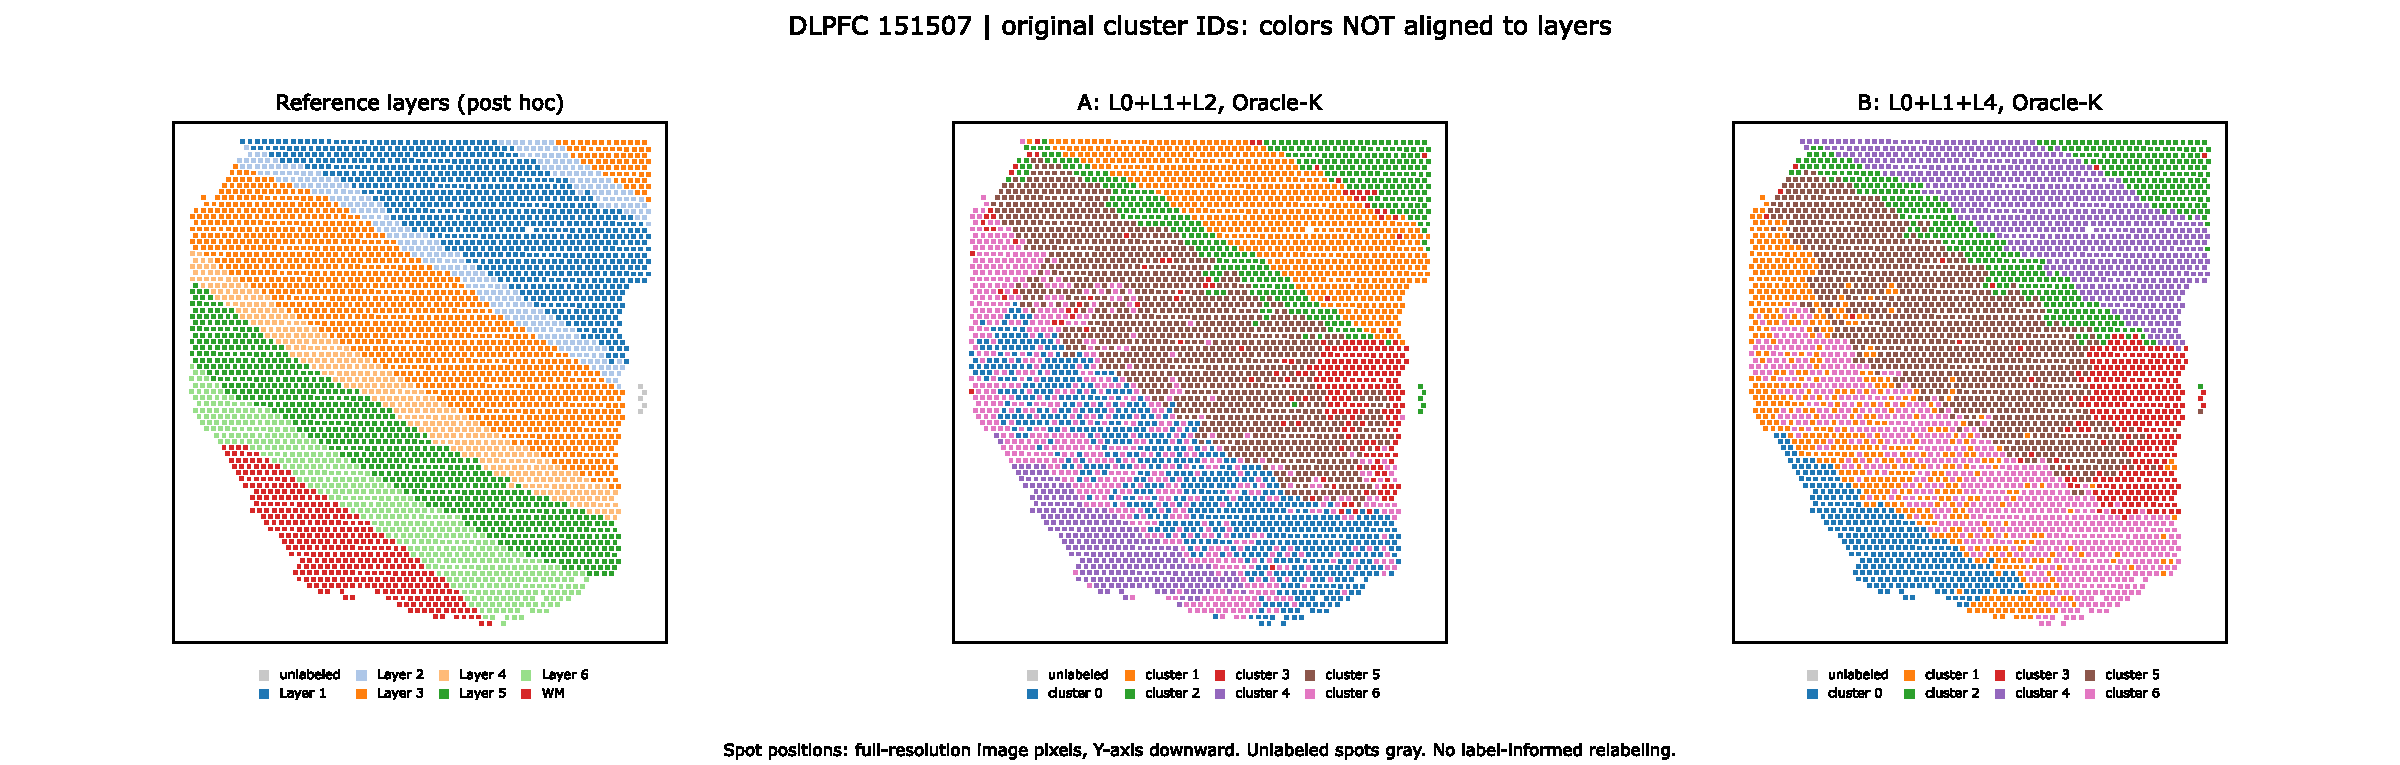
\includegraphics[width=0.98\linewidth]{E4_SOURCE_FIGURES_20261122_RELEASE/figures_pdf/151507/151507_reference_A_B_spatial.pdf}
\caption{DLPFC切片151507的参考组织层及冻结A15D、B15D原始聚类结果（E4真实SVG）。该切片按第一供体的B--A平均ARI正向代表规则选取；颜色不代表经过标签监督对齐的簇。}
\label{fig:cc-e4-151507-v1}
\end{figure}
}{%
\par\noindent\emph{[编译提示：未找到E4矢量PDF figures\_pdf/151507/151507\_reference\_A\_B\_spatial.pdf，请检查相对路径。]}\par
}
\IfFileExists{E4_SOURCE_FIGURES_20261122_RELEASE/figures_pdf/151671/151671_reference_A_B_spatial.pdf}{%
\begin{figure}[htbp]
\centering
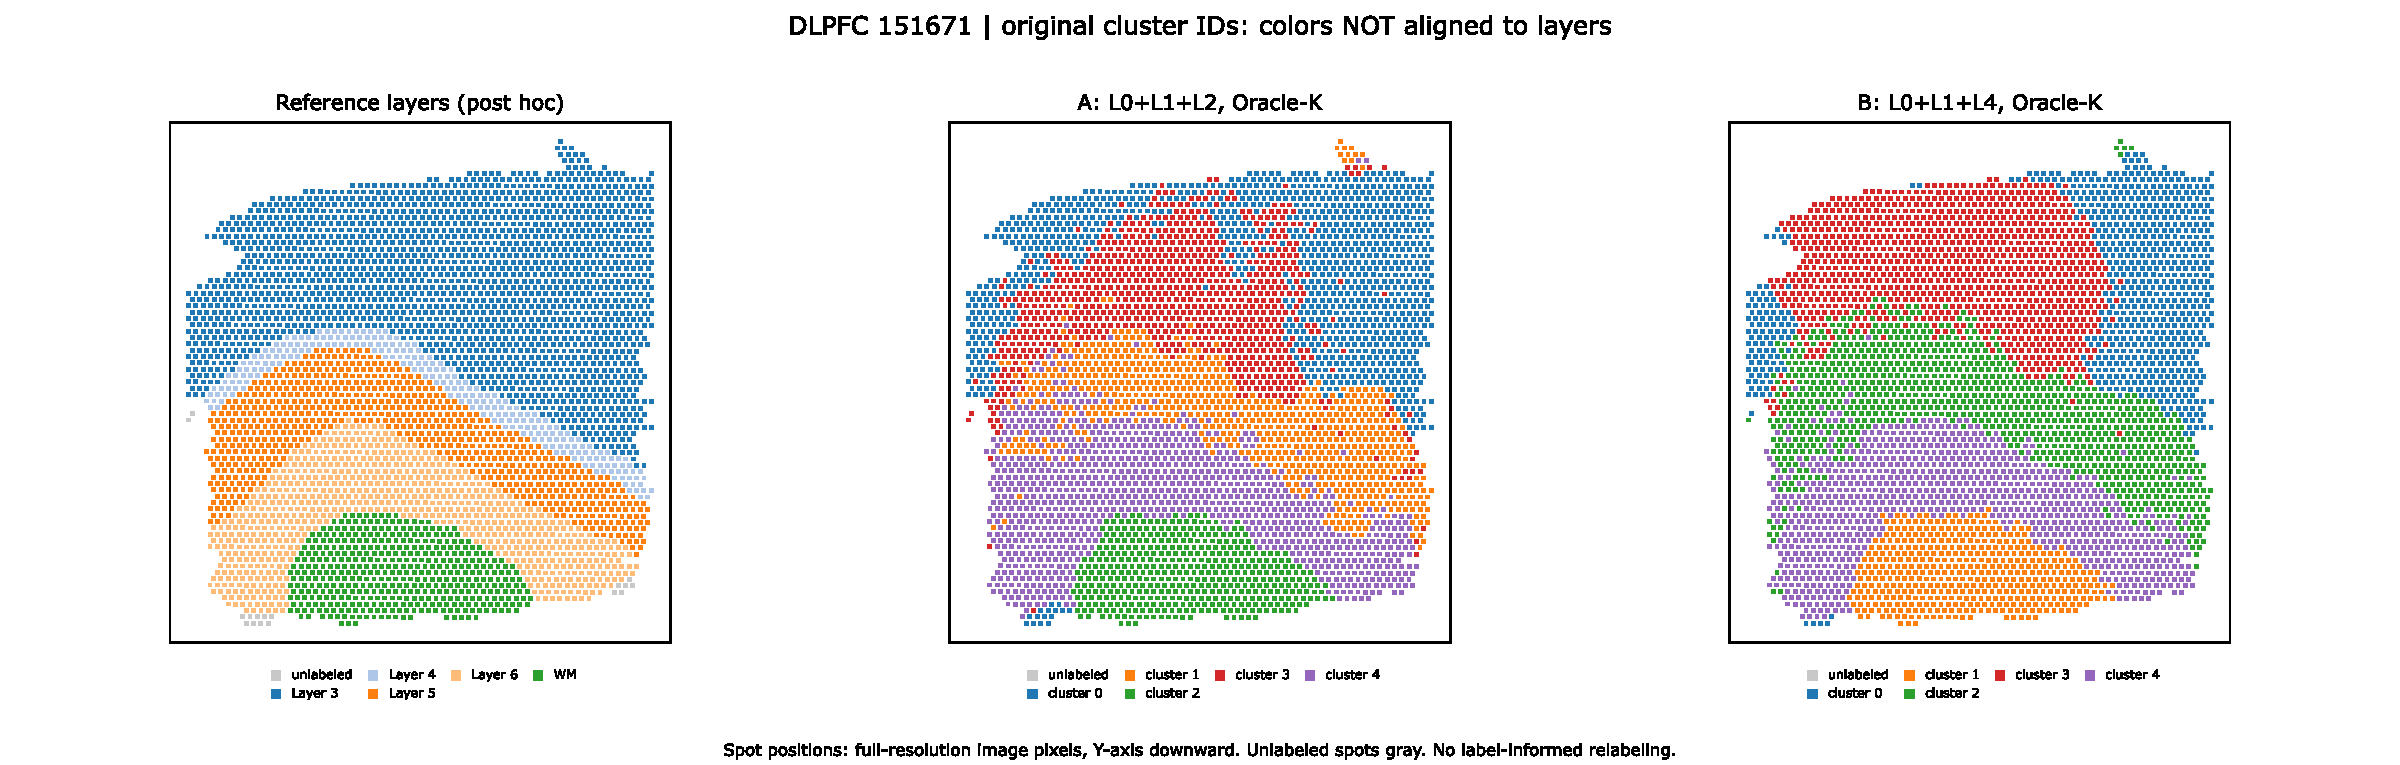
\includegraphics[width=0.98\linewidth]{E4_SOURCE_FIGURES_20261122_RELEASE/figures_pdf/151671/151671_reference_A_B_spatial.pdf}
\caption{DLPFC切片151671的参考组织层及冻结A15D、B15D原始聚类结果（E4真实SVG）。该切片按第二供体的B--A平均ARI接近零的规则选取。}
\label{fig:cc-e4-151671-v1}
\end{figure}
}{%
\par\noindent\emph{[编译提示：未找到E4矢量PDF figures\_pdf/151671/151671\_reference\_A\_B\_spatial.pdf，请检查相对路径。]}\par
}
\IfFileExists{E4_SOURCE_FIGURES_20261122_RELEASE/figures_pdf/151675/151675_reference_A_B_spatial.pdf}{%
\begin{figure}[htbp]
\centering
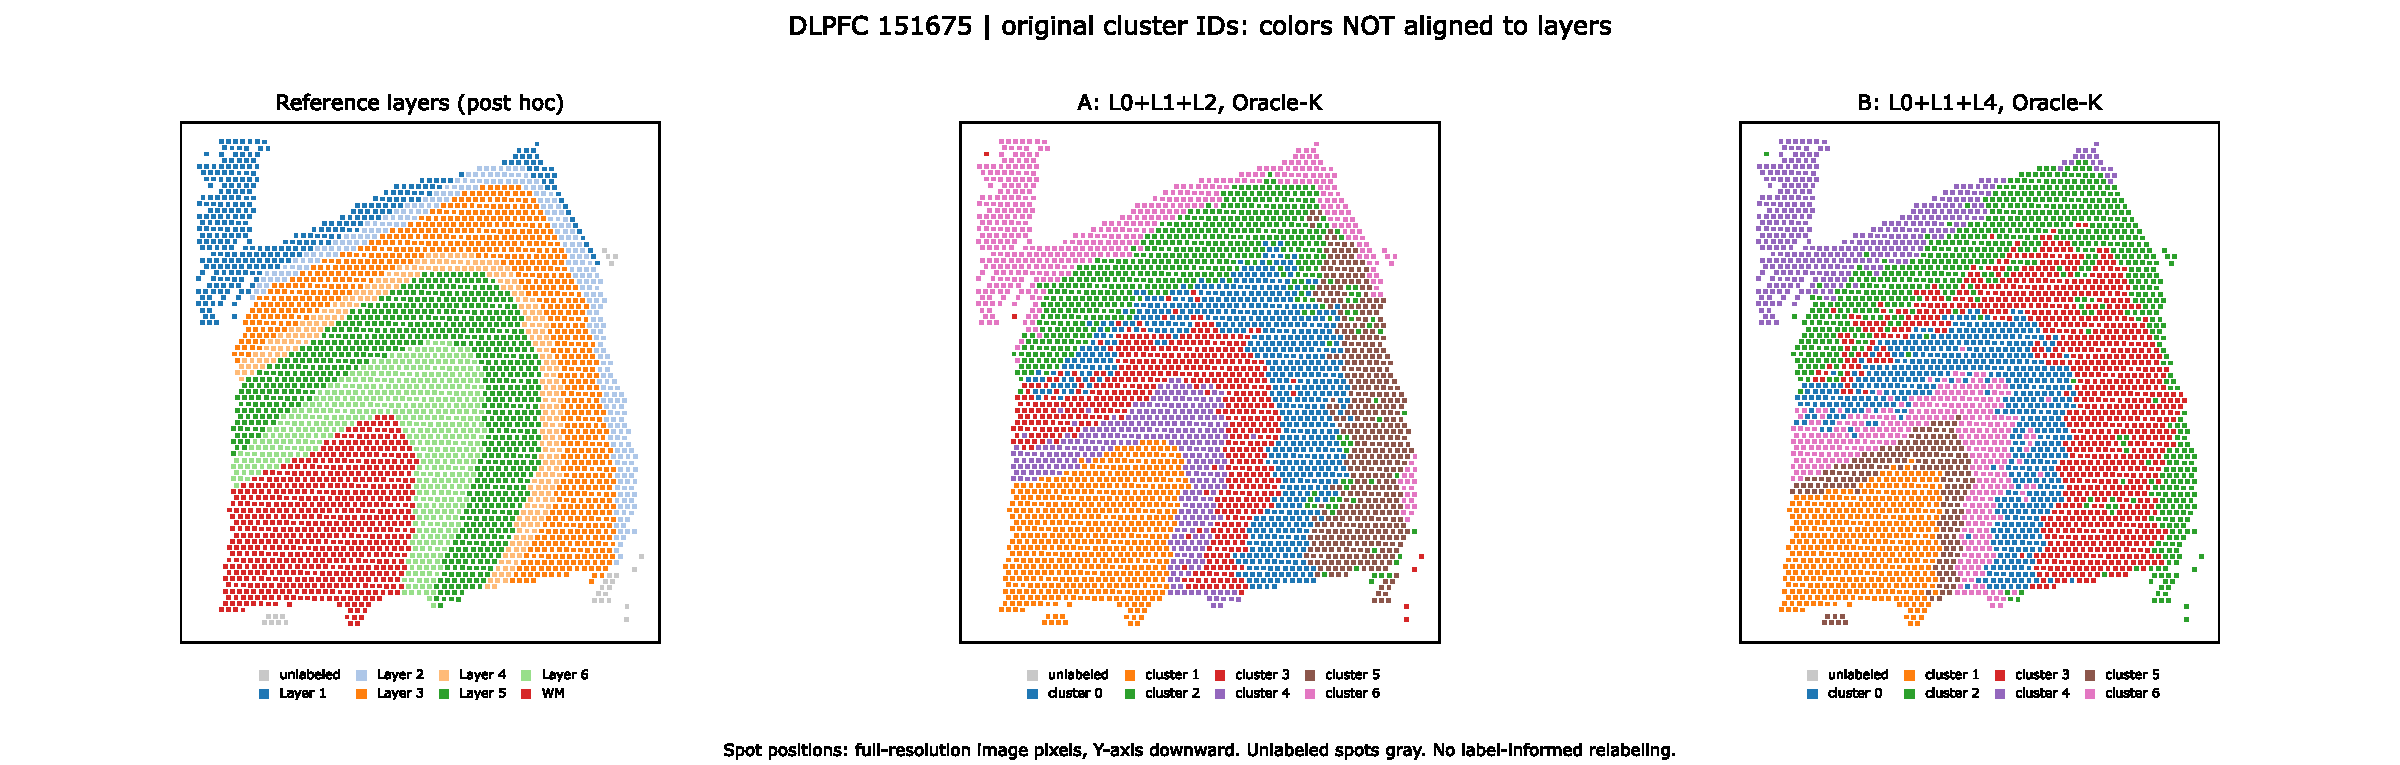
\includegraphics[width=0.98\linewidth]{E4_SOURCE_FIGURES_20261122_RELEASE/figures_pdf/151675/151675_reference_A_B_spatial.pdf}
\caption{DLPFC切片151675的参考组织层及冻结A15D、B15D原始聚类结果（E4真实SVG）。该切片按第三供体的B--A平均ARI负向代表规则选取。}
\label{fig:cc-e4-151675-v1}
\end{figure}
}{%
\par\noindent\emph{[编译提示：未找到E4矢量PDF figures\_pdf/151675/151675\_reference\_A\_B\_spatial.pdf，请检查相对路径。]}\par
}

为辅助理解皮层标记表达与空间域的关系，E4对每张切片的MOBP、PCP4、SNAP25三个标记基因分别从原始10x表达计数重新计算\texttt{log1p(10000$\times$基因UMI/spot总UMI)}，绘制统一颜色刻度范围0至6的表达图；对应原始与标准化数值保存在逐spot CSV。统一色标便于在图内比较表达分布，但图中的单个高表达区域不能直接作为人工组织层的独立验证，更不能证明某个聚类簇属于唯一确定的细胞类型。

\IfFileExists{E4_SOURCE_FIGURES_20261122_RELEASE/figures_pdf/151671/151671_MOBP_PCP4_SNAP25_expression.pdf}{%
\begin{figure}[htbp]
\centering
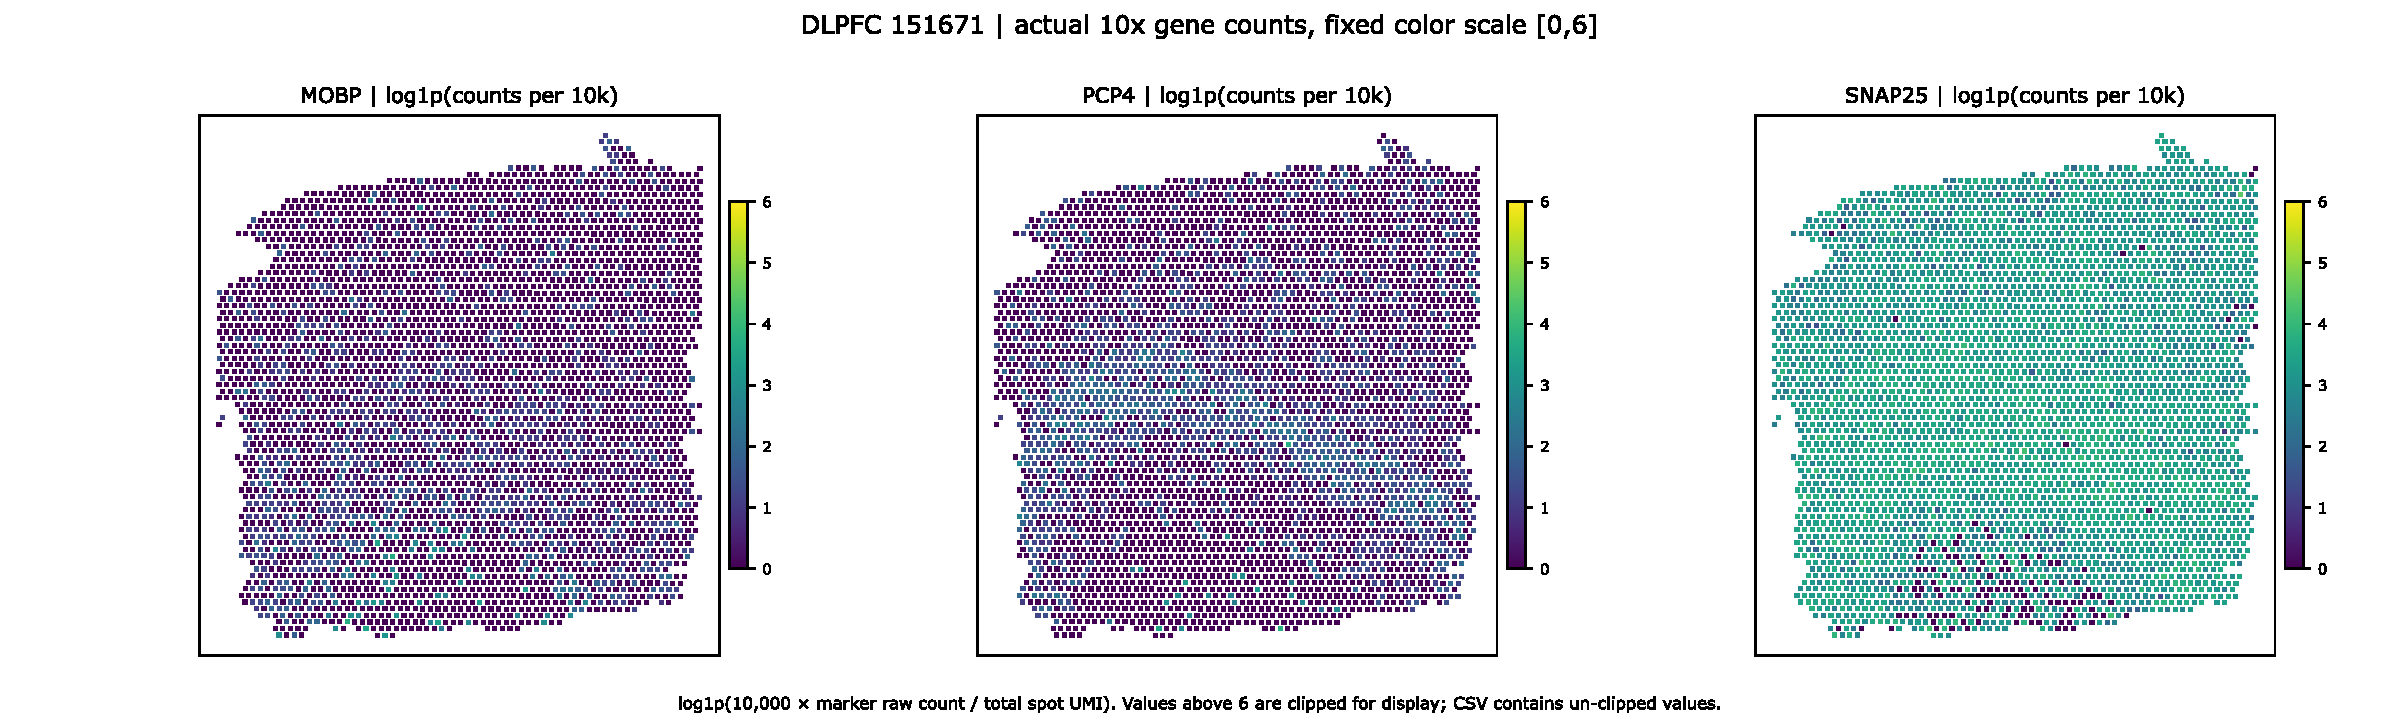
\includegraphics[width=0.98\linewidth]{E4_SOURCE_FIGURES_20261122_RELEASE/figures_pdf/151671/151671_MOBP_PCP4_SNAP25_expression.pdf}
\caption{DLPFC切片151671中MOBP、PCP4与SNAP25的原始计数归一化表达空间分布（E4真实SVG）。三图按相同归一化公式和0至6固定颜色范围展示。}
\label{fig:cc-e4-markers-151671-v1}
\end{figure}
}{%
\par\noindent\emph{[编译提示：未找到E4矢量PDF figures\_pdf/151671/151671\_MOBP\_PCP4\_SNAP25\_expression.pdf，请检查相对路径。]}\par
}

此外，E4对每张切片分别生成参考组织层与A15D/B15D原始聚类编号的完整计数交叉表及可视化，保留未标注spot的排除数量。交叉表反映不同真实层对应的聚类标签构成，避免在无监督聚类编号之间强行建立没有证据的一一对应关系。原E4独立审计报告12/12切片、36/36张SVG及36/36份CSV的产物完整性与输入SHA一致，并重新校核了marker计数和交叉表。全部36张原始SVG及其派生矢量PDF已归档，并列于附录。本章目前只把E4用作对聚类分布的直观补充，尚未对图中具体的组织形态或局部marker模式作定量陈述；若补写这类观察，须以对应的逐spot CSV和交叉表为依据。

早期旧稿曾用151671与151676举例说明单种子下边界F1正负方向的差异；此处新E4图示固定的三张代表切片遵循另一套已记录的切片级\textbf{平均ARI}代表规则，不应将这两套事后案例选择依据混同。
 

\subsection{综合讨论及本章小结}
\label{subsec:cellcharter-discussion-v1}

本章的实证结果从以下几个方面说明，多尺度空间特征聚类的评价不能仅依据单一ARI均值。

第一，25D配置及2--4层的比较与CellCharter原作者的DLPFC调参和基准重叠；本研究25D的宏平均ARI与官方单切片结果处于同一水平，但由于重复结构、GMM参数、输入文件和版本不同，这不构成严格复现。

第二，在已冻结的Oracle-K与10个技术种子条件下，5D到10D的提升在全部切片中一致；15D之后，宏平均只略有上升，约半数切片和供体D3方向相反。在固定K网格中，宏平均的尺度排序稳定。开发切片上提名的等维候选B，在其余切片和外部K-blind条件下没有复现其优势。

第三，无标签AutoK选出的簇数随切片和尺度变化很大，与参考类别数一致的情况很少。由于只做了5次重复且逐切片运行，这一结果不能直接等同于原作者推荐设置下的表现。事后ARI/NMI显示尺度表现不是简单的单调关系。

第四，严格边界F1主要随recall变化，而recall又与预测分区的碎片化程度（预测边界数量）密切相关；严格F1与1/2-hop容差F1的排序相反，不能单独用其中一个指标判断边界定位精度。

成熟基线及外部队列进一步揭示了结果的适用边界。A15D相对5D和非空间基线在6名外部患者中方向一致，但在3名ARI低于0.05的患者中差值很小。与BayesSpace的比较存在指标方向不一致的问题，并且BayesSpace和GMM的K-blind似然判据都存在明显的搜索上界问题；在Oracle-K下，A15D的ARI低于BayesSpace和Leiden。对照集也未包含原文中单切片表现最好的STAGATE。上述结论支持把本项工作定位为\textbf{基于成熟CellCharter流程、在原作者DLPFC基准之上扩展的多尺度与选K敏感性、空间边界评价及外部复核的系统实证评价}，而不是将已知特征聚合方法包装为新的基础算法。

本研究的限制主要包括：（1）DLPFC仅3名独立供体，且供体映射依据公开附录推定分组，仍需与原始元数据进一步核对；乳腺癌外部队列为6例患者，不宜作高精度群体推断。（2）25D配置由原作者在151507、151672、151673上按参考标签调出，候选B在开发切片151507上提名，这些切片都不是未接触样本。（3）部分实验使用标签类别数知情的Oracle-K，不能称为纯无监督选K表现。（4）不同空间方法的输入表征与计算路径并非完全相同；BayesSpace与GMM的K-blind判据频繁命中上界，其中BayesSpace判据与官方建议不一致；对照集未包含STAGATE。（5）AutoK每个候选K只做5次稳定性重复，未做收敛检查，且逐切片运行。（6）邻域深度和输入维度共同变化，不能据此确定因果性空间平滑机制；边界分析没有零模型基准。（7）E3d事后评分、E3b边界与容差指标、排除开发切片的汇总以及与官方结果的对照，都是在看过既有结果后进行的分析，不能倒称为前瞻注册的主终点或独立验证。（8）技术种子标准差只反映GMM初始化变异，不是生物学重复。（9）用于展示的组织学标注具有数据集特定性，外部队列并非医学诊断金标准。

综上，在遵守数据来源、独立生物学单位和完整负结果报告的前提下，现有实验已经形成从固定尺度、K敏感性、严格与容差边界到成熟基线和外部组织数据的完整描述性证据链。后续论文章节应以真实实验记录、可复算结果和可核实文献说明研究贡献，不对尚未证明的算法创新或普遍性能优势作过度推断。
